
\section{Introduction}

GPS devices are widely used in orchard planting and maintenance. This location-based system allows orchardist to check trajectory of tractors. The trajectory is a connection by a time series successive positions recorded by GPS devices. A classical GPS device records skeleton information, including time mark, latitude, longitude, number of available satellites, etc. Recently, researchers try to enrich trajectory (called Semantic Trajectory) by adding background geographic information to discover meaningful pattern \cite{ying2011semantic}. 


Normally GPS units record more data than necessary and cause more errors due to weak signals or shelter from branches. To obtain a higher accurate observation dataset and to same local storage space, several data simplification methods were proposed and are focusing on simplifying data set by making either a local or global decision. 

A local simplification algorithm focuses on a couple of particular consecutive points. By analyzing the relationship between these points, a decision is made that which point can be deleted or retained. Distance threshold algorithm is one of these algorithms. All points, for which the distance to the preceding track point is less than a predetermined threshold is deleted. Direction changing algorithm is another one. The point is retained if the change in direction is greater than a predetermined threshold  \cite{ivanov2012real}. 

Alternatively, global simplification algorithms have an overview of all tracked points. After analyzing the relationships among these points, a decision will be made about which one or more points to delete or to retain. The Douglas-Peucker algorithm is the most popular one  \cite{douglas1973algorithms}. A proposed simplification method, represented in \cite{chen2009trajectory}, consider both the skeleton information and semantic meanings of a trajectory when performing simplification. 


Intuitively, the global simplification algorithms can be applied on off-line data analyses and local simplification algorithms will perform better on on-line or real-time track simplification. However, a pertinent algorithm is required in our case. 


In our case, a GPS log is a sequence time series points $p_i \in P$, $P=\{ p_1,p_2, \ldots, p_n \}$. Each GPS point $p_i$ contains information of time mark, latitude, longitude and semantic information of velocity, heading direction and boom status, which can be written in form of
\begin{equation}
T=\{p_t=[x_t,y_t,v_t,\theta_t,b_t] \mid t \in \mathbb{R} \}.
\end{equation}
Sequentially connect these points will give us a trajectory of a moving vehicle.
Particularly, a tractor working on an orchard generates two kinds of boom status information: working and not working. This information is recorded by GPS units and is indicated by $b=1$ for working and $b=0$ for not-working.


To move further, here are two concepts that will be useful to understand the simplification scheme.
\begin{itemize}
\item $\mathbf{Segment}$ A segment is a part of the consecutive trajectory. Regarding the status of the boom, the trajectory can be simply divided into two kinds of the segment in our dataset, one is boom-working, the other is boom-not-working. 
\item $\mathbf{Direction}$. Direction $\theta$ denotes the heading direction of a tractor at a specific point location. This parameter uses north direction as a basis, in which way $\ang{0} \leq \theta < \ang{360}$.
\end{itemize}



\section{Simplification Algorithm}

The first two steps are designed to reduce some errors caused by misoperation and GPS units bugs.
\begin{itemize}
\item Merging Phase. If the length of a segment composed of consecutive boom working or not-working points is less than a threshold, merge this one into its backward segment. 
\item Removing Phase. If two or more data points have duplicated time mark, remove the latter ones. 
\end{itemize}
Now only two types of segment points are left in GPS log, boom working, and not-working and the length of each segment are greater than the predetermined threshold.

The following algorithm is based on the relationship between a candidate point $p_i$ and it's neighboring points $p_{i-1}$ and $p_{i+1}$, and the importance of the $p_i$ in the segment where it belongs to, $i=2,\ldots,n-1$. 

\begin{itemize}
\item Rule 1. The candidate point $p_i$ is retained if it is not linear predictable or cannot be used for linear predicting. With the velocity information $v_{i-1}, v_i$ at point $p_{i-1}, p_i$ and time differences $\Delta t_{i-1} = \lvert t_{i}-t_{i-1} \rvert,\Delta t_{i} = \lvert t_{i+1}-t_{i}\rvert$, an estimated position can be calculated by $\hat{p}_i=\Delta t_{i-1} p_{i-1}$, $\hat{p}_{i+1}=\Delta t_{i} p_{i}$. If the distance $\lvert \hat{p}_i-p_i\rvert$ or $\lvert \hat{p}_{i+1}-p_{i+1}\rvert$ is less than a threshold, then the point $p_i$ is not linear predictable or cannot be used for linear predicting.

\item Rule 2. Select a candidate point $p_i$. Retain this point if the distance between $p_i$ and $p_{i-1}$ is greater than the threshold $d$, where $d$ is the mean distances of these points $p_{i-1}, p_i, \ldots, p_{i+k}$ with same boom status $b_{i-1}=b_i=\cdots=b_{i+k}$. 

\item Rule 3. Neighbor Heading Changing. The candidate point $p_i$ belongs to the track if $\lvert \theta_i-\theta_{i-1}\rvert  + \lvert \theta_i-\theta_{i+1}\rvert >\theta$, where $\lvert \theta_i-\theta_{i-1}\rvert$ and $ \lvert \theta_i-\theta_{i+1}\rvert $ are the direction changes between points $p_i$ and $p_{i-1}$ and between points $p_i$ and $p_{i+1}$, $\theta$ is predefined threshold.

\item Rule 4. The candidate point $p_i$ belongs to the track if the boom status $b_i\neq b_{i-1}$.
\end{itemize}

Finally, the point $p_i$ belongs to the track if Rule 1 = TRUE or Rule 2 = TRUE or Rule 3 = TRUE or Rule 4 = TRUE.


\section{Evaluation}

Errors are measured by Synchronized Euclidean Distance \cite{lawson2011compression}. SED measures the distances between the original and compressed trace at the same time. As shown in figure \ref{DataSimpSED}. $P_{t1}, \ldots ,P_{t5}$ are original points. After simplification, the points $P_{t2}, P_{t3}$ and $P_{t4}$ were removed. The black curve is the original trajectory, in contrast, gray dash line is the simplified trajectory. The gray point $P'_{t2}$ on simplified trajectory has the same time difference as the point $P_{t2}$ on original trajectory does. Then the distance between $P_{t2}$ and $P'_{t2}$ is calculated.


\begin{figure}[h]
\centering
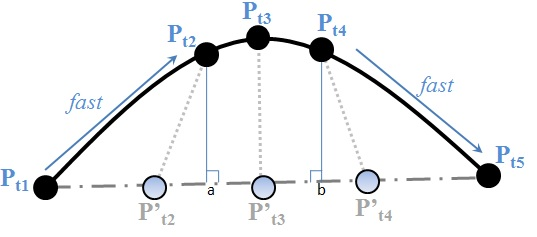
\includegraphics[width=0.9\textwidth]{Chapters/06Spinoff/plot/sed.jpg}
\caption{Synchronized Euclidean Distance \cite{lawson2011compression}}\label{DataSimpSED}
\end{figure}

Another way to calculate the difference between a GPS trace and its compressed version is to measure the perpendicular distance. This algorithm ignores the temporal component and uses simple perpendicular distance. The figure \ref{DataSimpAB} expresses these difference clearly. 

\begin{figure}[h]
\centering
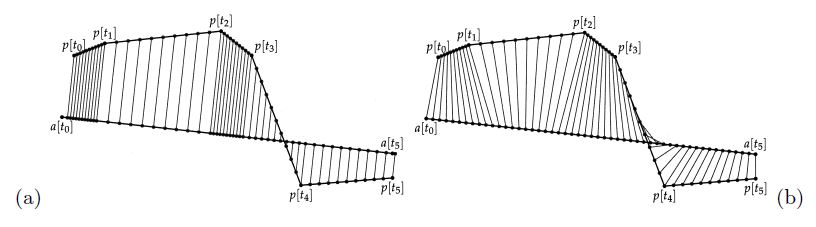
\includegraphics[width=0.9\textwidth]{Chapters/06Spinoff/plot/ab.JPG}
\caption{(a) error measured at fixed sampling rate as sum of perpendicular distance chords; (b) error measured at fixed sampling rates as sum of time-synchronous distance chords. \cite{meratnia2004spatiotemporal}}\label{DataSimpAB}
\end{figure}


\section{Numerical Study}

In the numerical simulation study, we are using Kalman Filter (KF) to fit the trajectory after data simplifying. The KF equations describe the prediction step in the following way: 
\begin{align*}
\hat{x}_k^-&=A\hat{x}_{k-1}+Bu_k \\
P_k^-&=AP_{k-1}A^\top+Q
\end{align*}
where $\hat{x}_k^-$ is a priori state estimate, $\hat{x}_k$ is a posteriori state estimate, $A$ is status transition matrix, $P_k^-$ is a priori estimate for error covariance, $u_k$ is an input parameter and $Q$ is process noise covariance. 

When a new observation comes into the data stream, KF update and corrects its estimation by: 
\begin{align*}
K_k&=P_k^-H^\top (HP_k^-H^\top+R)^{-1} \\
\hat{x}_k&=\hat{x}_k^-+K_k(z_k-H\hat{x}_k^-) \\
P_k&=(I-K_kH)P_k^-
\end{align*}
where $K_k$ is the Kalman gain matrix, $z_k$ is the observed data.


The original data set has 1021 rows, each of them contains latitude, longitude, velocity, bearing (heading direction) and boom status. Douglas-Peucker Algorithm, with distance threshold $0.205$m, retained 847 points. The proposed algorithm, given a predictable distance $5$m and heading direction changing threshold $\ang{30}$, returns the same amount of simplified points. Under the same circumstance, we calculated SED and other information. 

Table (\ref{DataSimpCompTable}) describes the results after simplifying by DP algorithm and the proposed algorithm. Figure \ref{DataSimpRawTra} demonstrates the simplified raw data and figure \ref{DataSimpKFTra} is the fitted trajectories by Kalman filter. 

\begin{table}
\centering
\caption{Comparison between raw data and simplifying algorithms}
\label{DataSimpCompTable}
\begin{tabular}{|l|c|c|c|}
\hline 
  & \textbf{Original Data} & \textbf{DP Algorithm} & \textbf{Proposed Algorithm}  \\
\hline 
\textbf{Points Left} & 1021              & 847         & 847         \\
\textbf{Tracked Distances}(m)  & 74041.31     & 74038.33    & 74012.56     \\
\textbf{SED} (m)    & NA        & 1316.715    & 607.9587   \\
\hline 
\end{tabular}
\end{table}


\begin{figure}[h]
\centering
%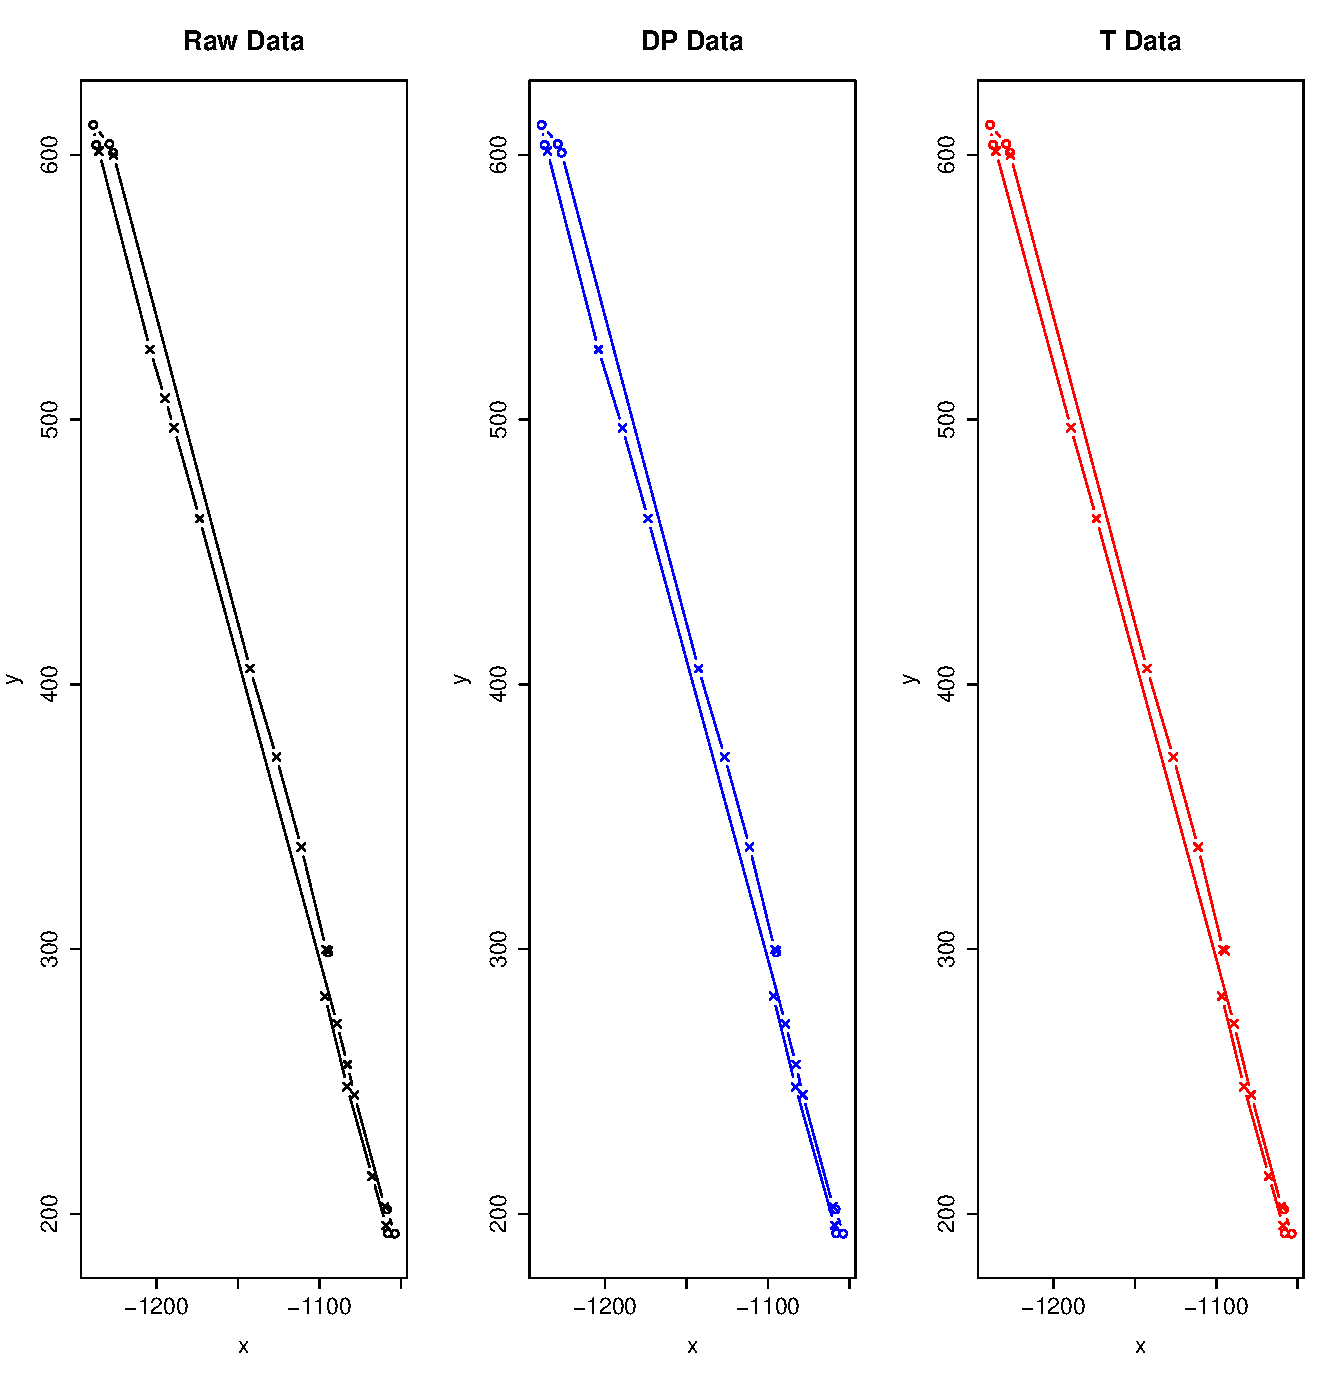
\includegraphics[width=0.9\textwidth]{Chapters/06Spinoff/plot/3p1.pdf}
\begin{subfigure}[t]{0.47\textwidth}
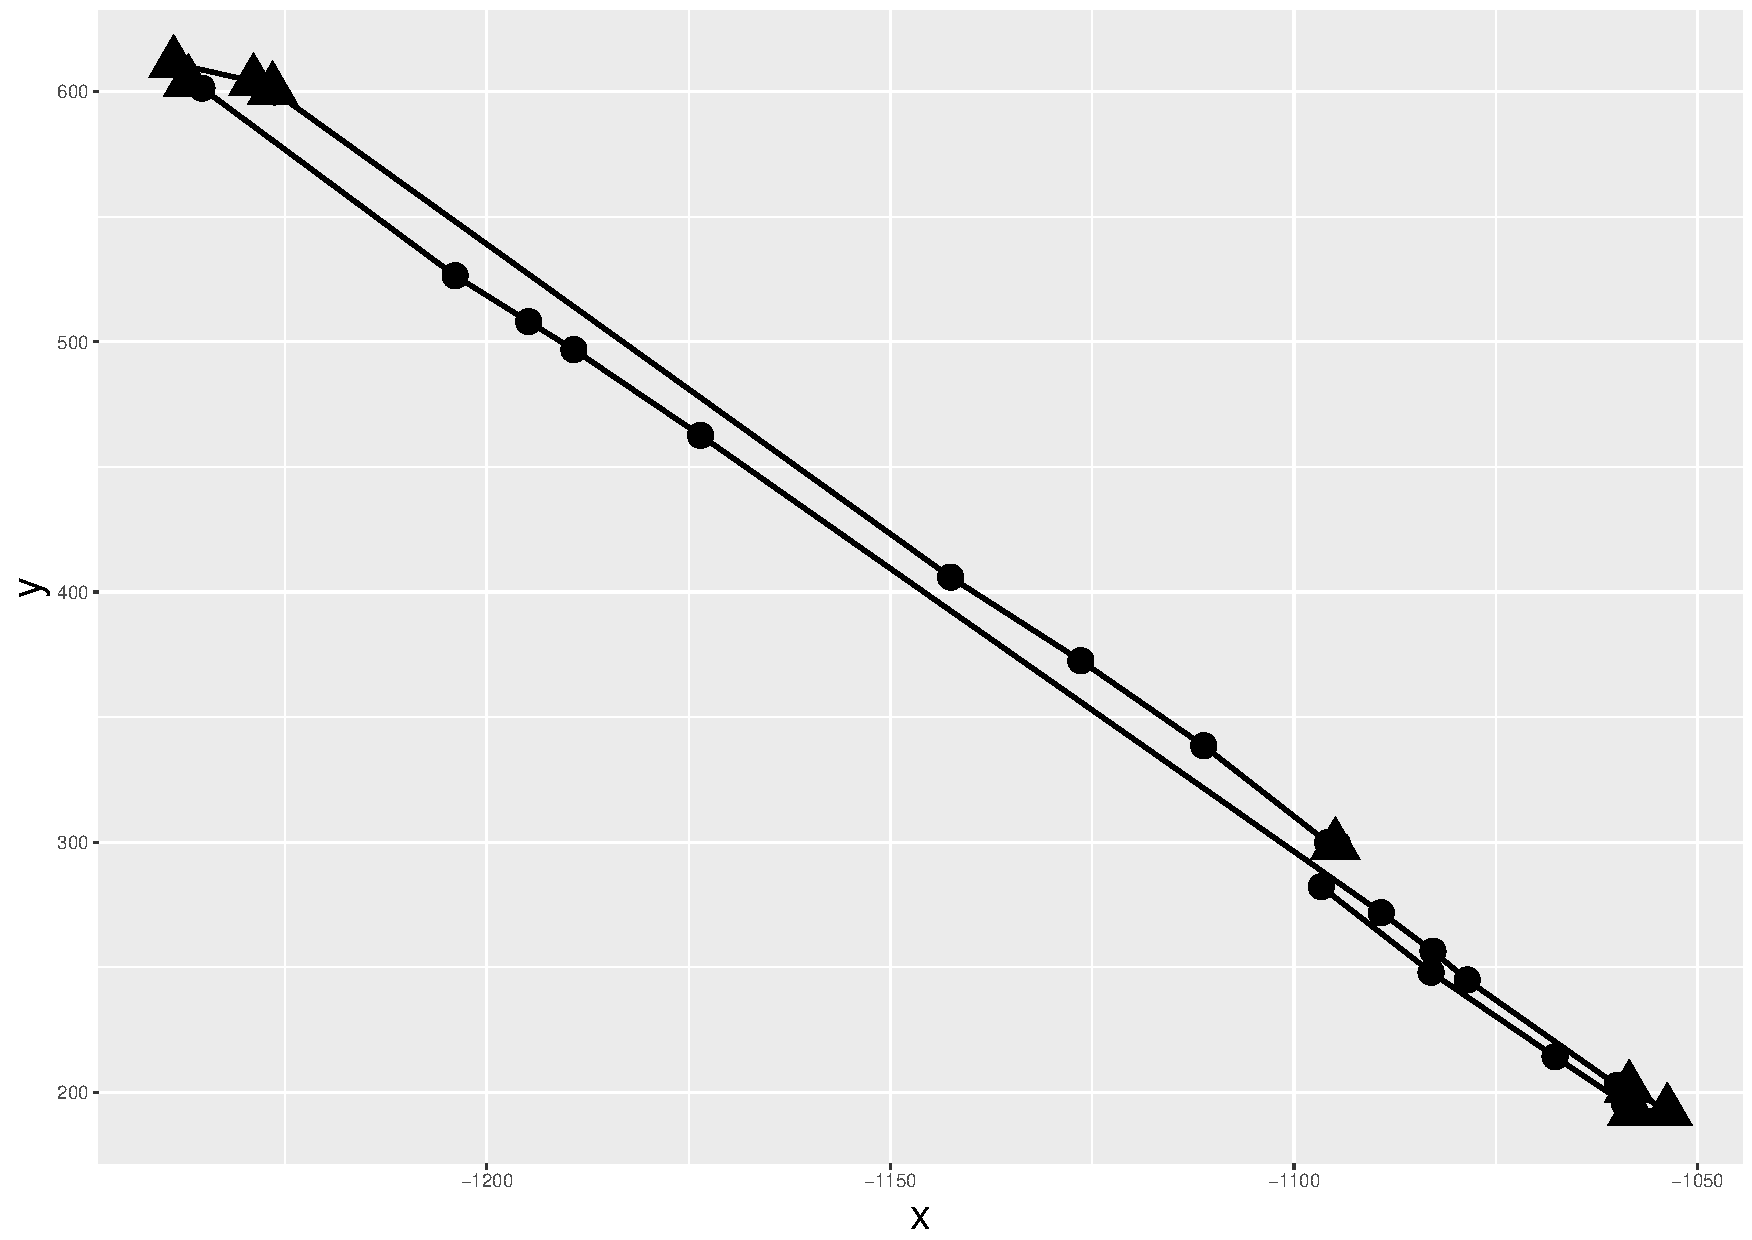
\includegraphics[width=\linewidth]{Chapters/06Spinoff/plot/ggRawTrac.pdf}
\caption{Raw trajectory}
\end{subfigure}
 \begin{subfigure}[t]{0.47\textwidth}
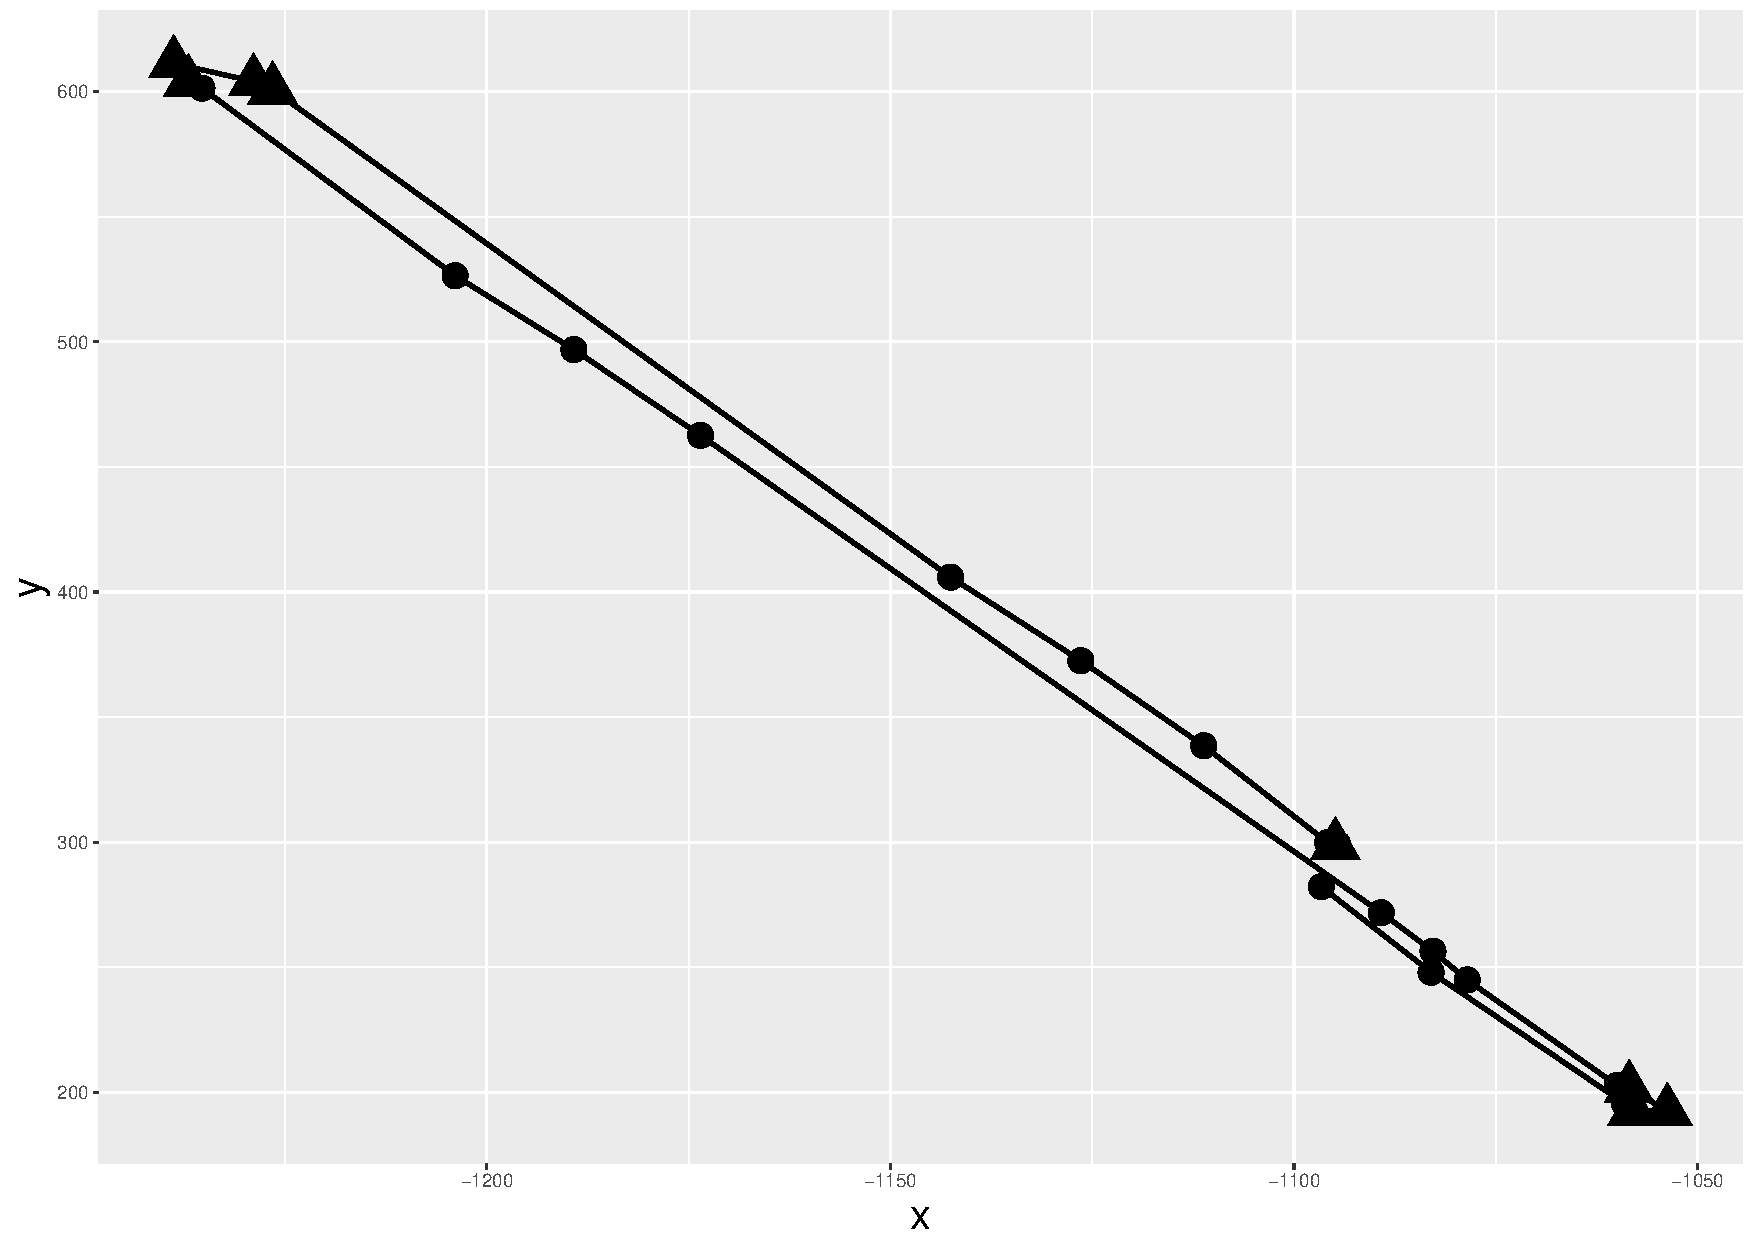
\includegraphics[width=\linewidth]{Chapters/06Spinoff/plot/ggDPTrac.pdf}
\caption{Simplified trajectory by DP}
\end{subfigure}
 \begin{subfigure}[t]{0.47\textwidth}
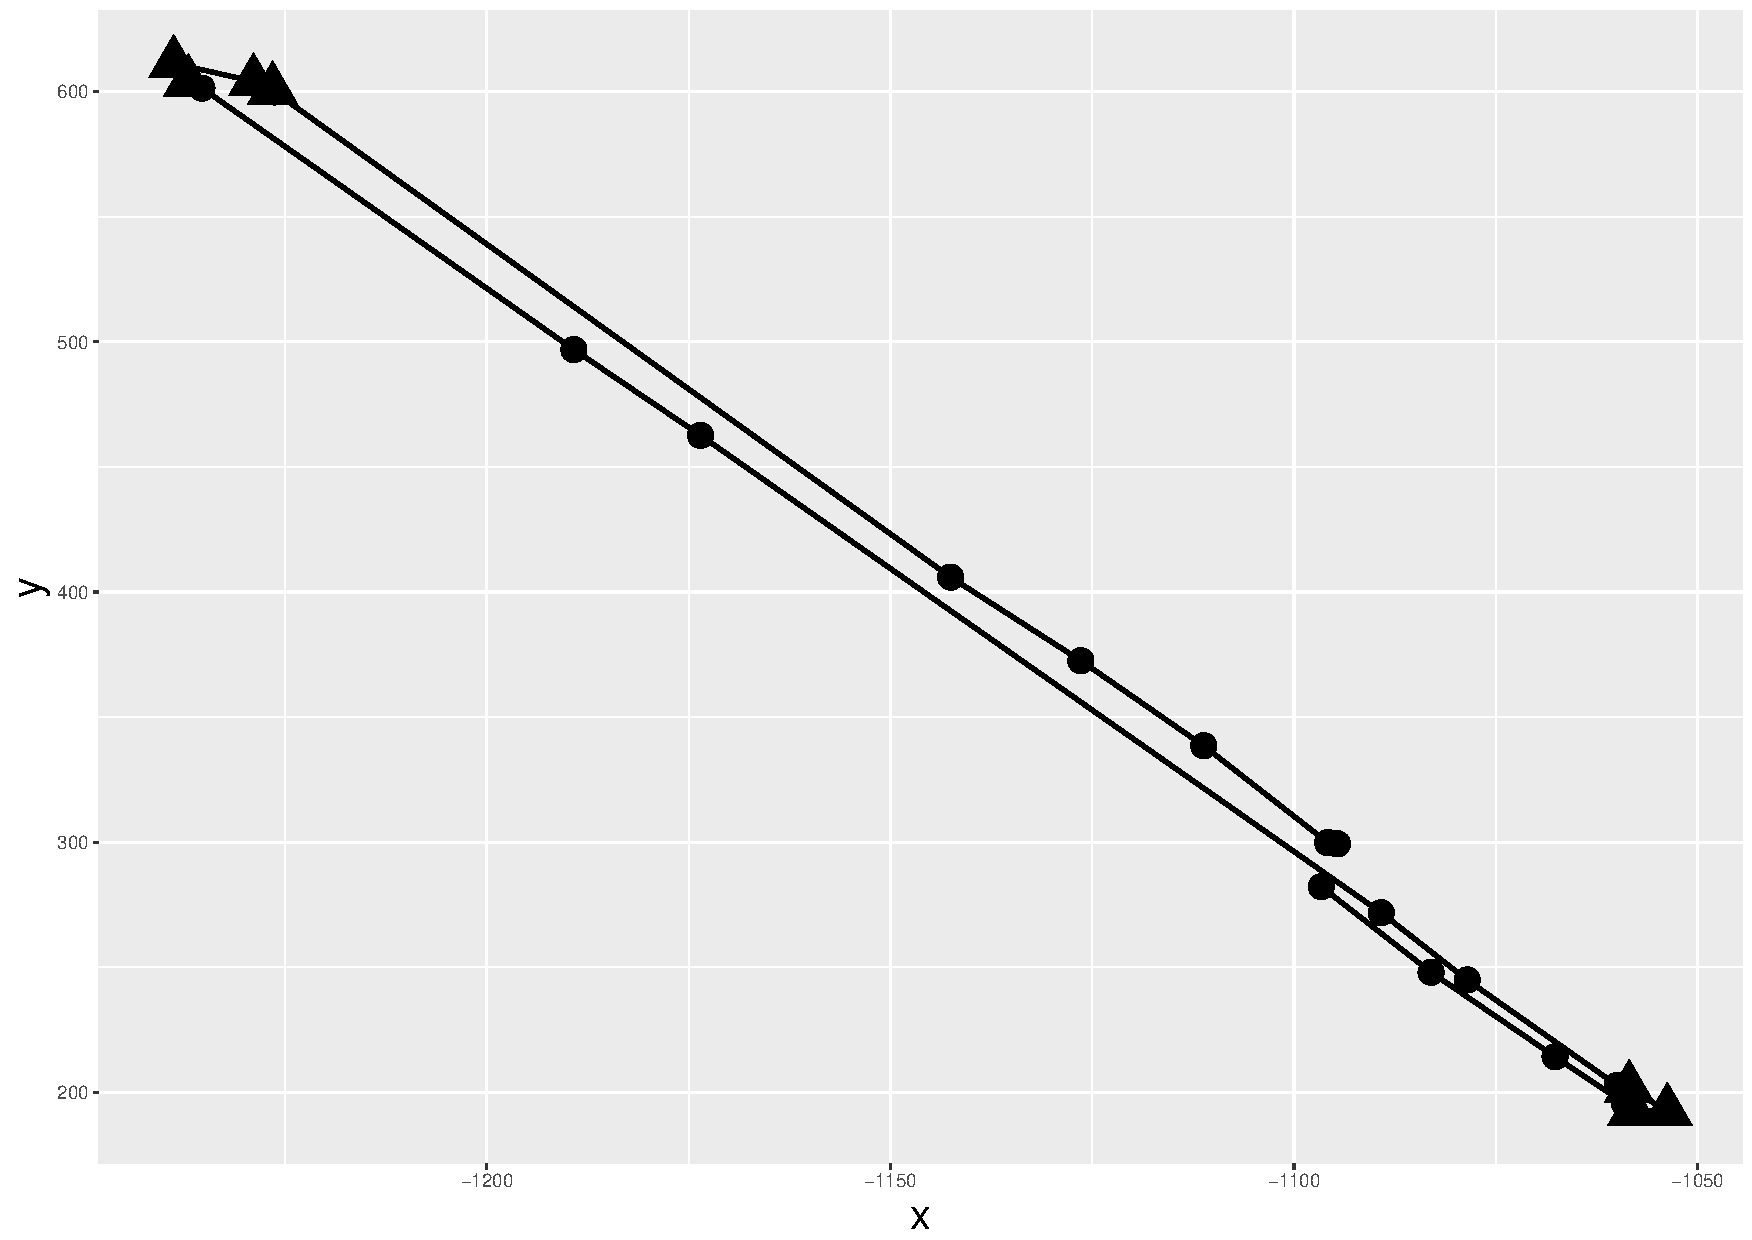
\includegraphics[width=\linewidth]{Chapters/06Spinoff/plot/ggSPTrac.pdf}
\caption{Simplified trajectory by proposed algorithm}
\end{subfigure}
\caption{A segment start from time $t=2000$ to $3000$, recorded by GPS units. $\blacktriangle$ indicates the boom is not-working. $\bullet$ indicate the boom is working. Figure (a), it's the trajectory connected by raw data with 27 points. Figure (b), it's the trajectory connected by simplified data with Douglas-Peucker algorithm with 24 points. Figure (c), it's the trajectory connected by simplified data with proposed simplification algorithm with 23  points.}\label{DataSimpRawTra}
\end{figure}

\begin{figure}[h]
\centering
%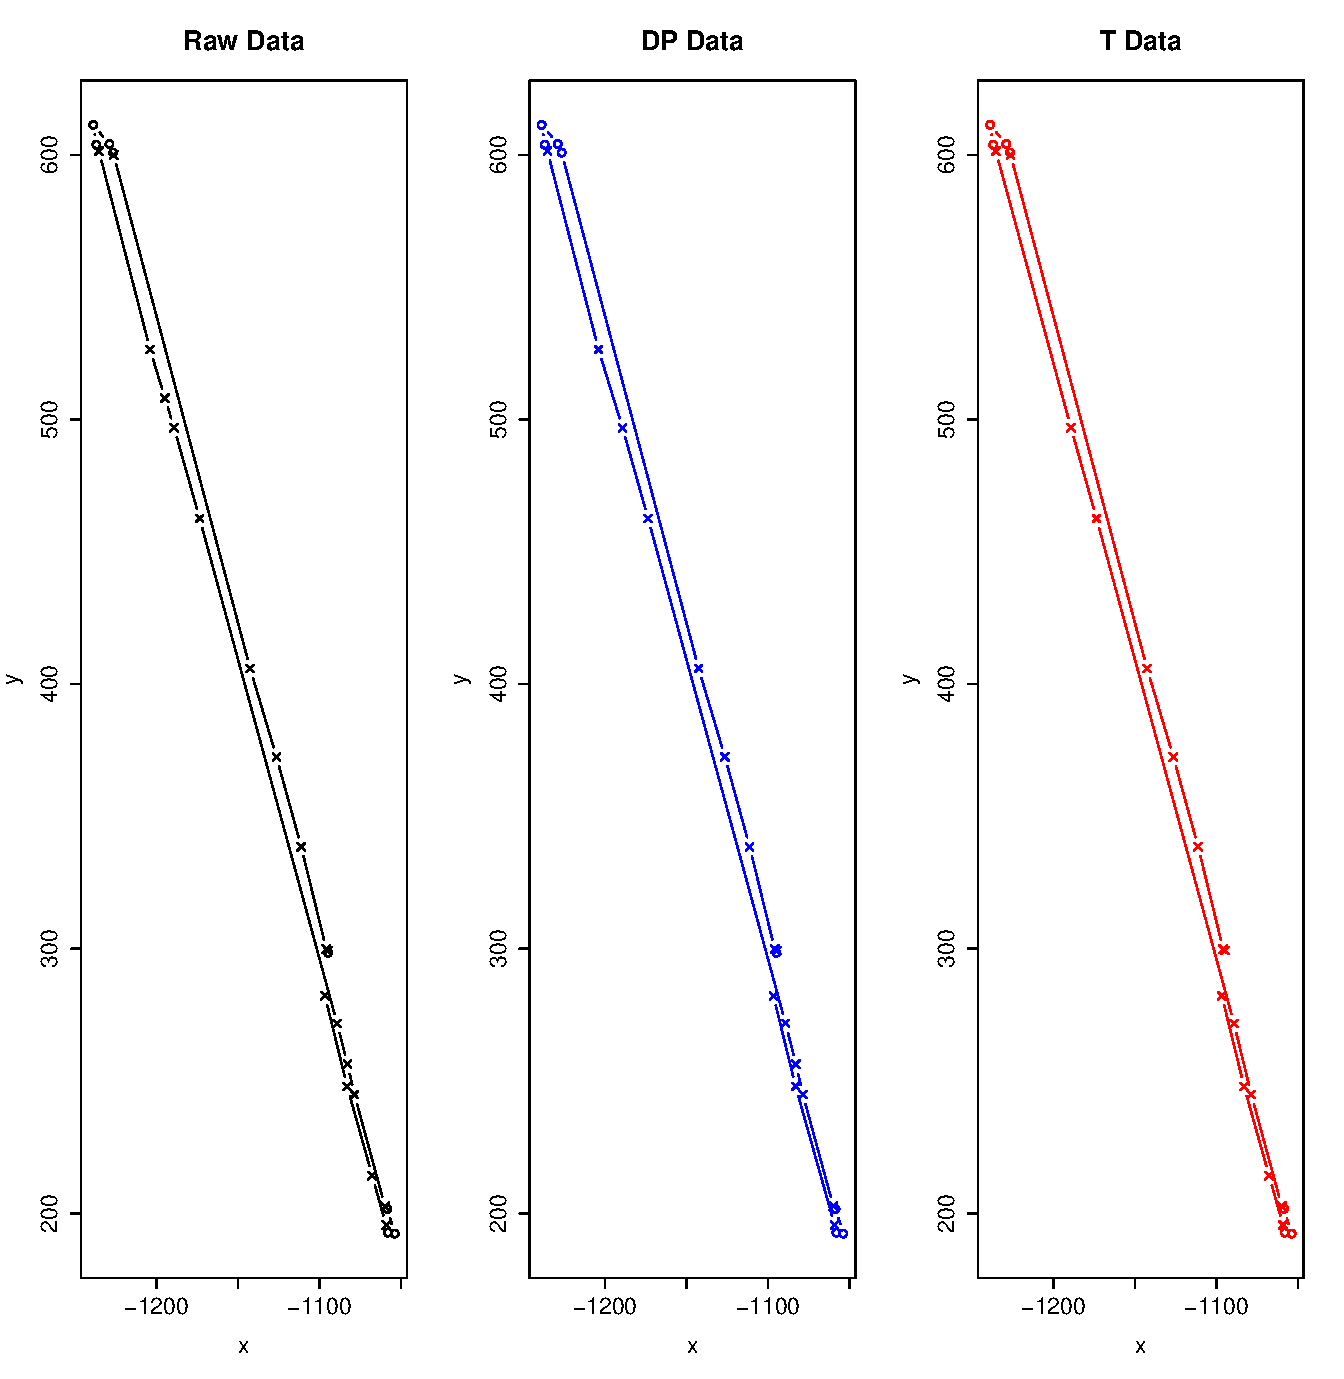
\includegraphics[width=0.9\textwidth]{Chapters/06Spinoff/plot/km3p}
\begin{subfigure}[t]{0.47\textwidth}
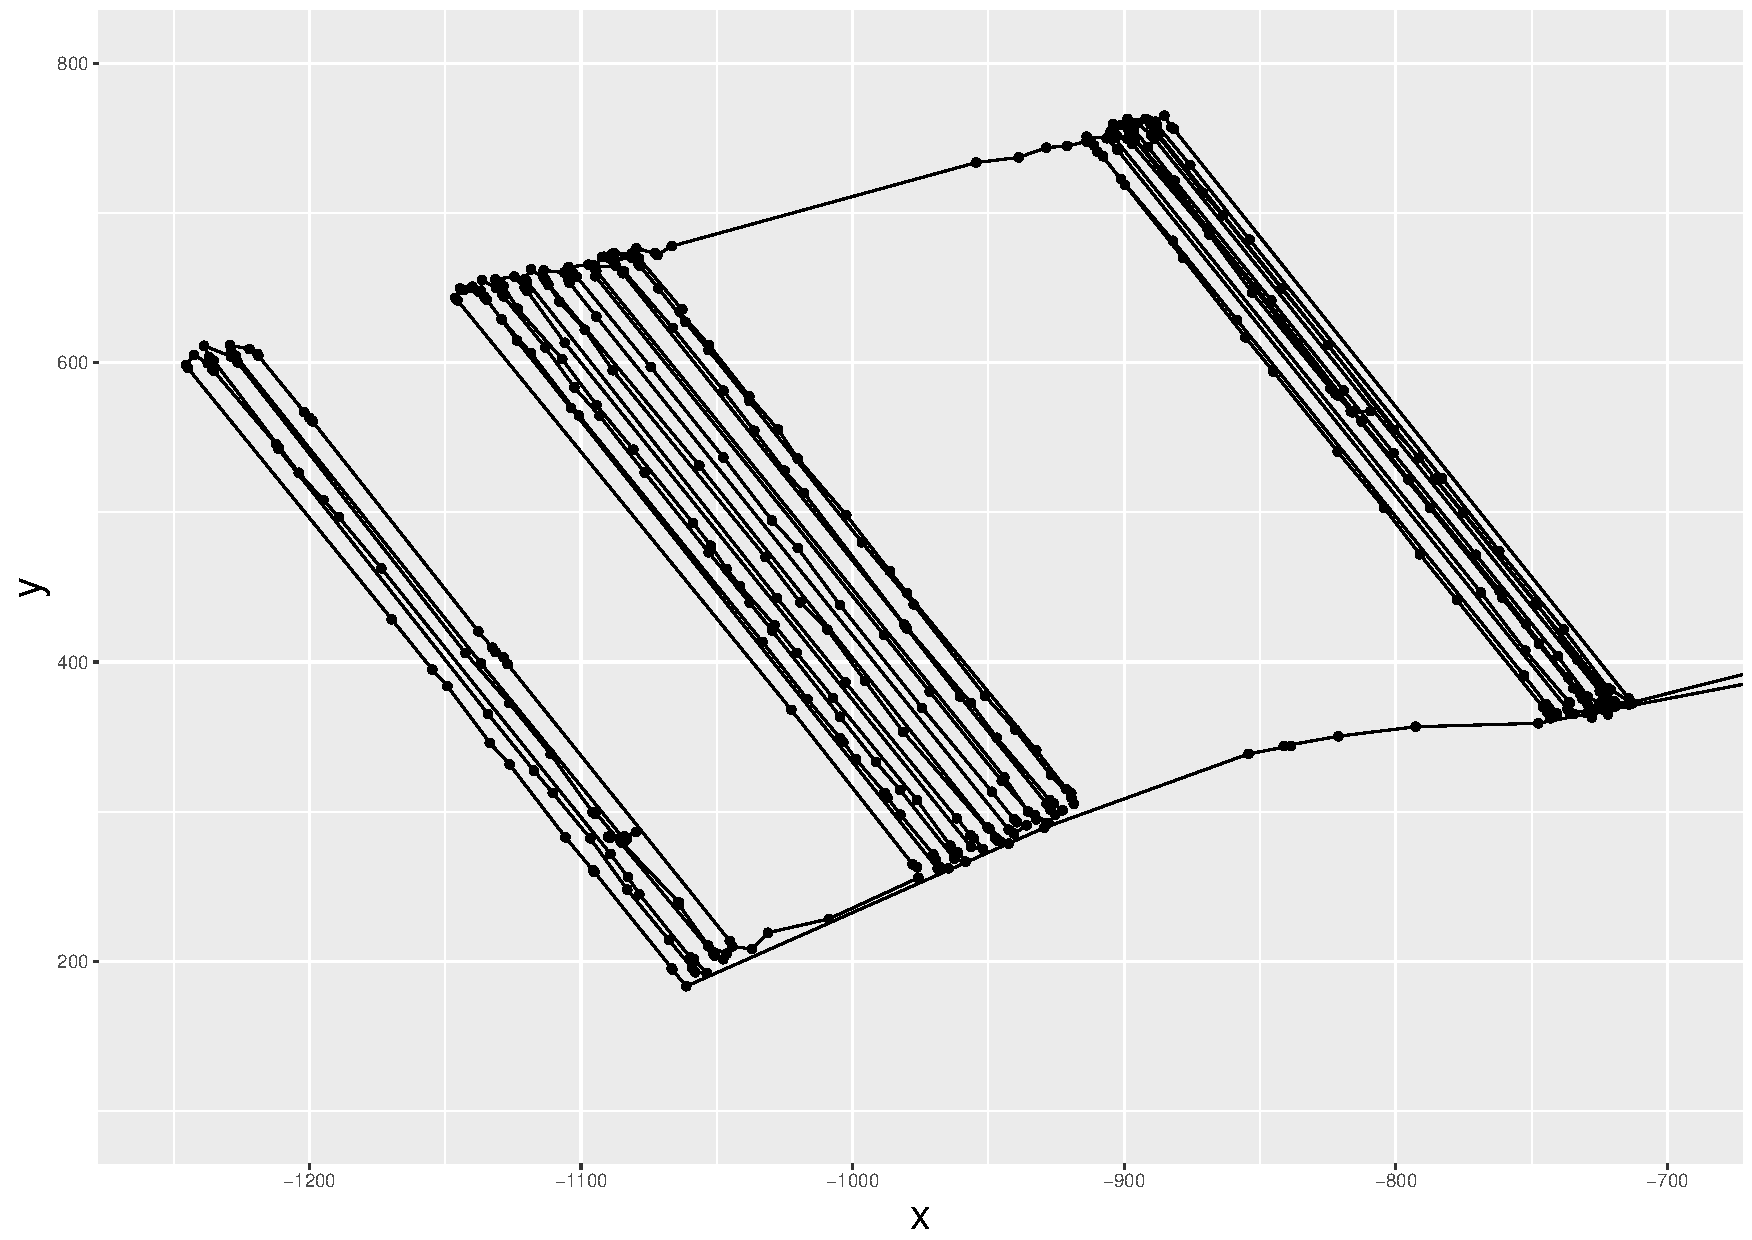
\includegraphics[width=\linewidth]{Chapters/06Spinoff/plot/ggRawKF.pdf}
\caption{Fitted Kalman Filter with raw data}
\end{subfigure}
 \begin{subfigure}[t]{0.47\textwidth}
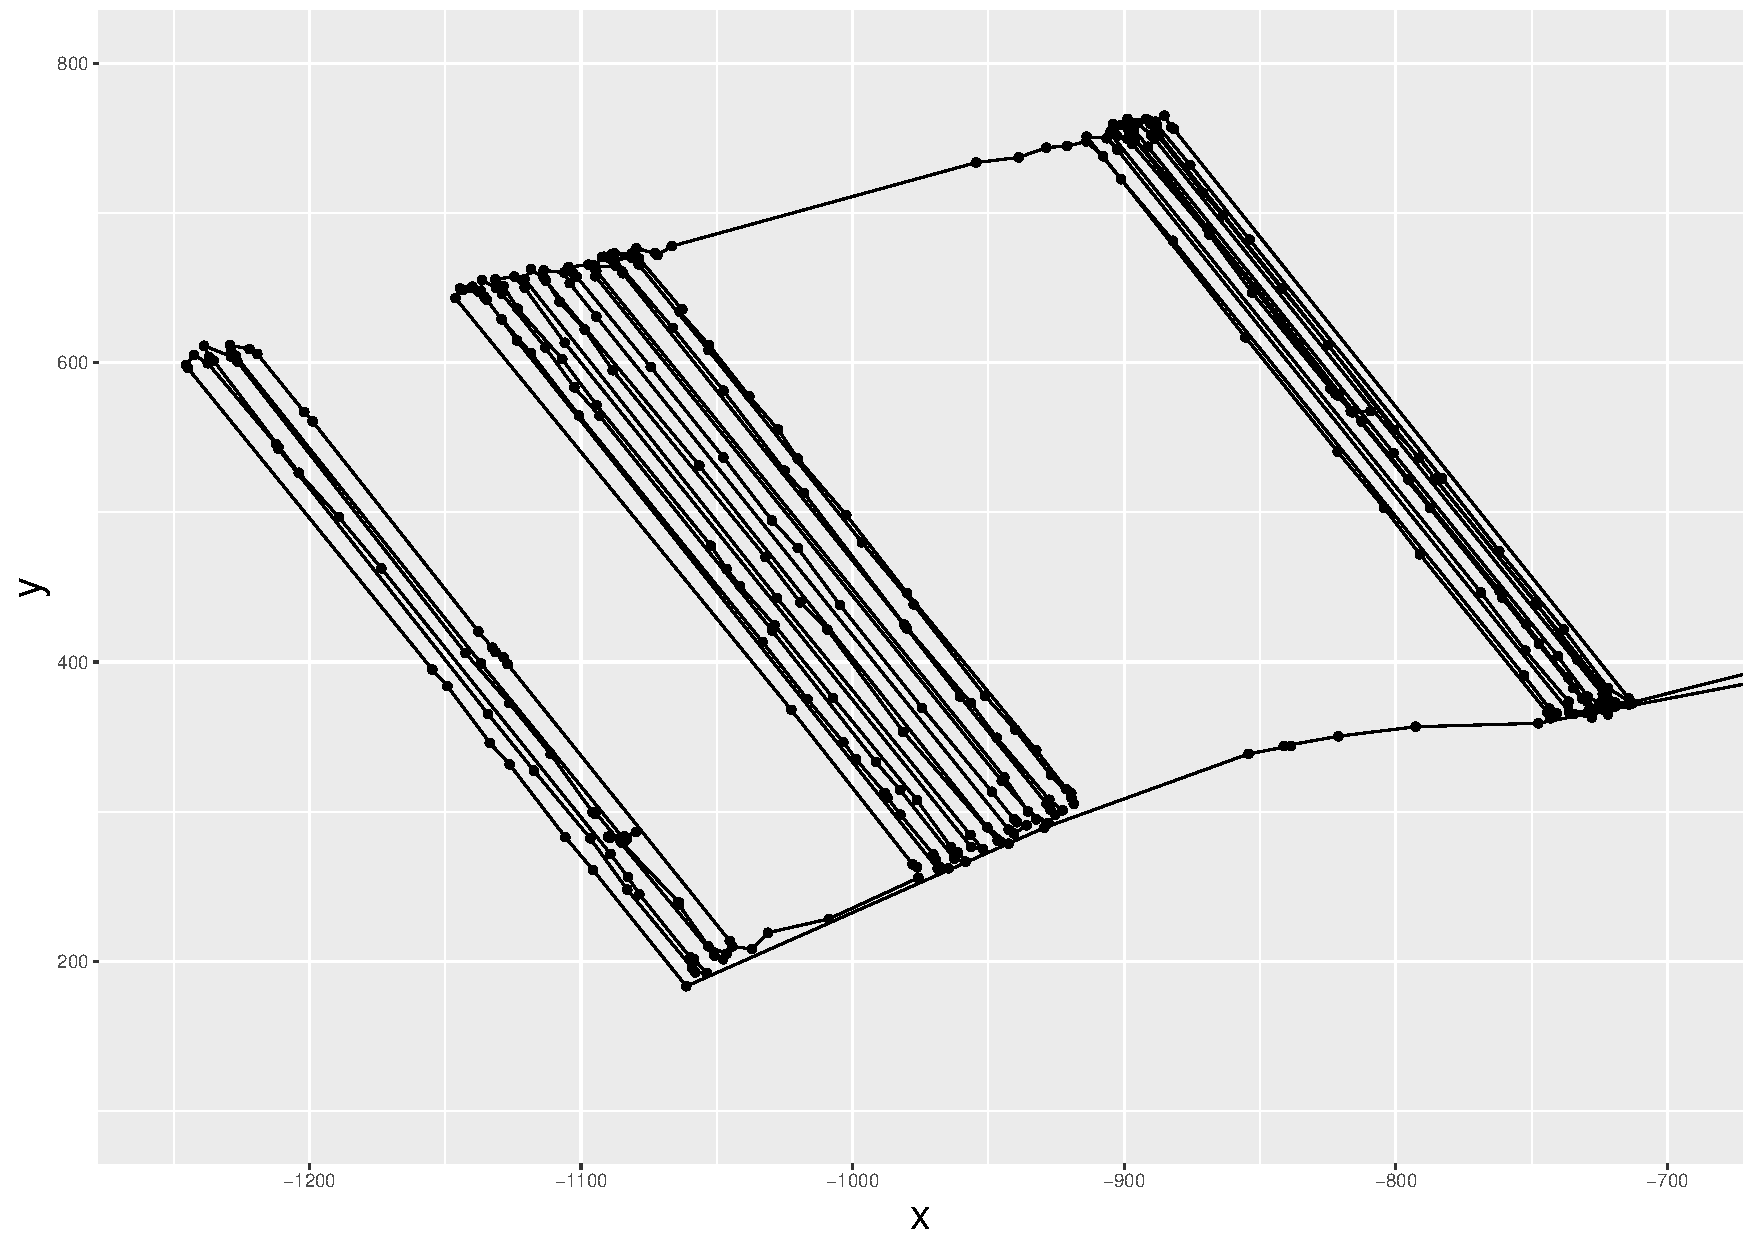
\includegraphics[width=\linewidth]{Chapters/06Spinoff/plot/ggDPKF.pdf}
\caption{Fitted Kalman Filter with simplified data by DP}
\end{subfigure}
 \begin{subfigure}[t]{0.47\textwidth}
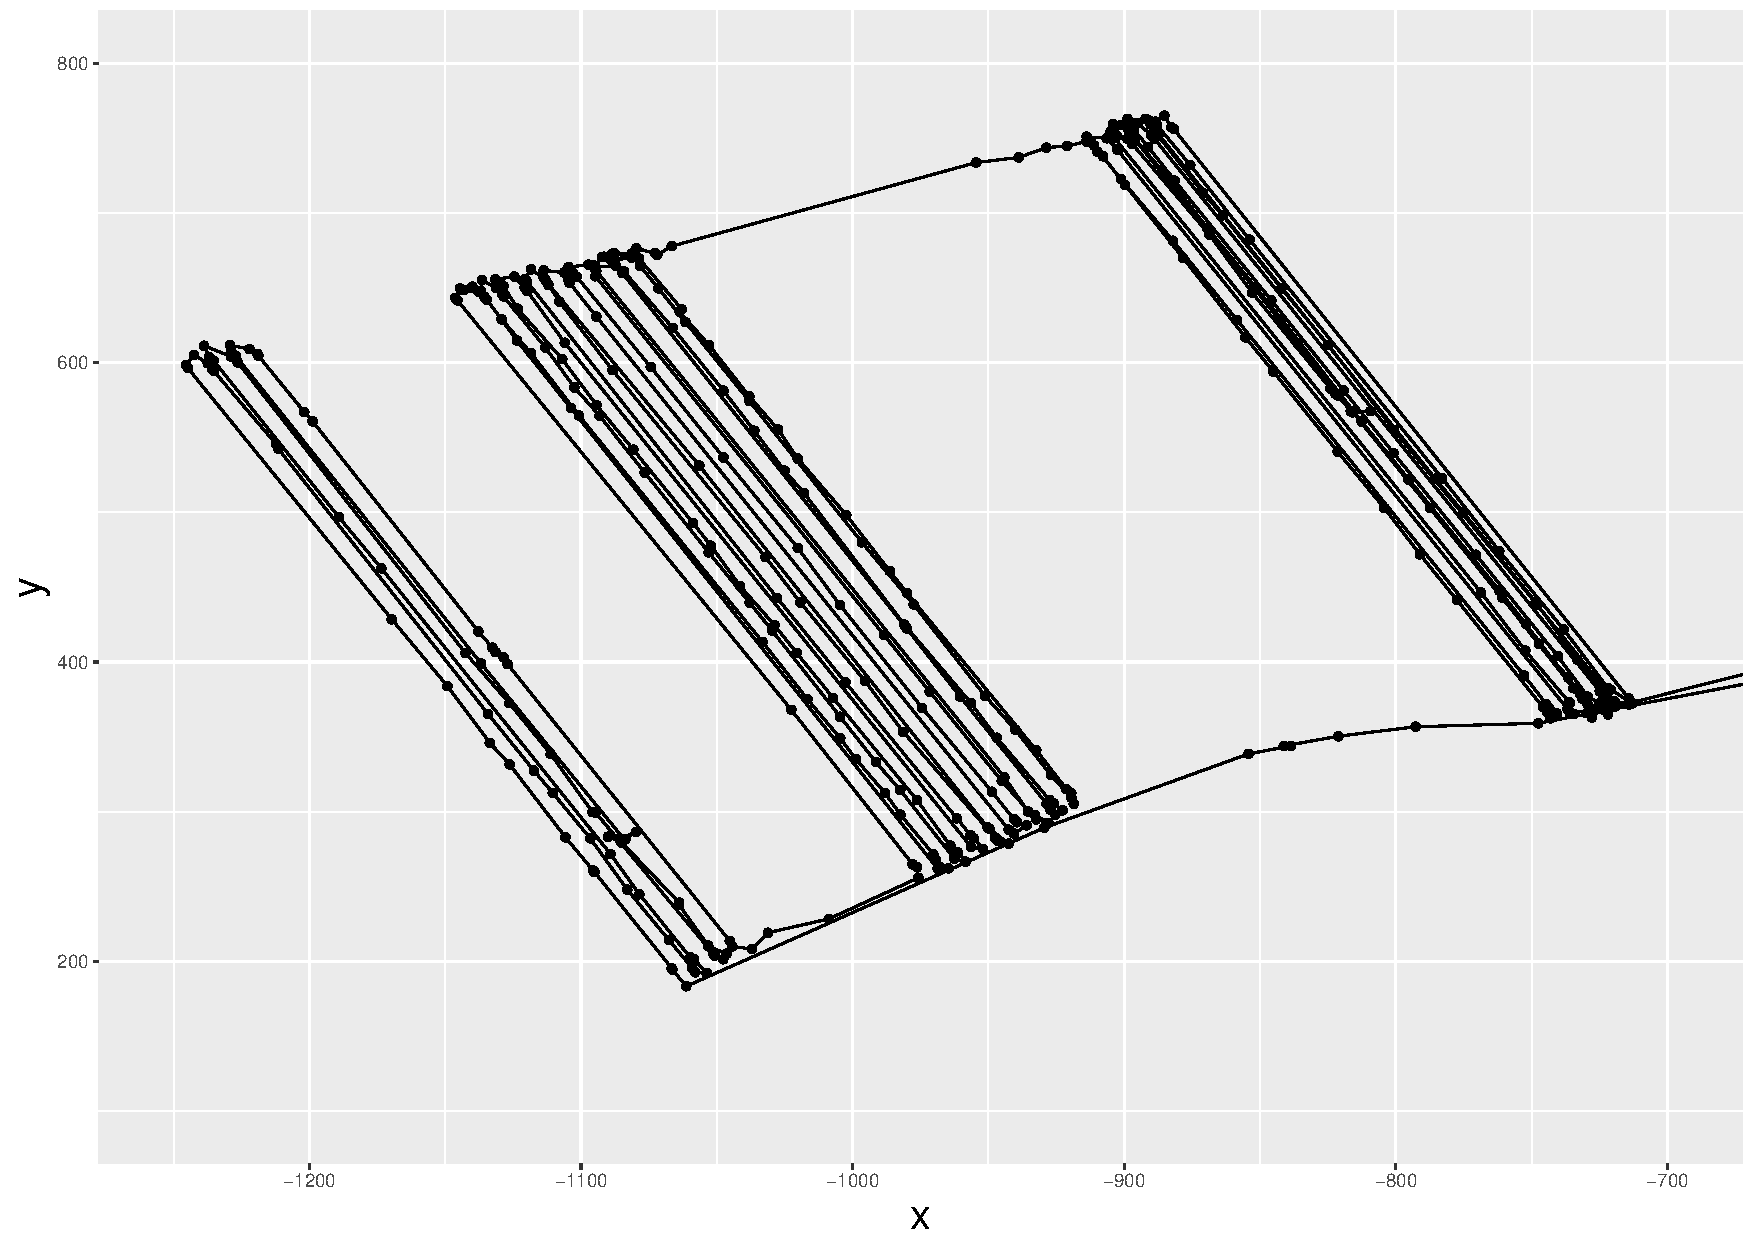
\includegraphics[width=\linewidth]{Chapters/06Spinoff/plot/ggSPKF.pdf}
\caption{Fitted Kalman Filter with simplified data by proposed algorithm}
\end{subfigure}
\caption{Trajectory fitted by Kalman Filter. The mean squared errors of raw data, DP and proposed algorithm are 26.8922, 23.9788 and 23.9710 respectively.}\label{DataSimpKFTra}
\end{figure}


\section{Conclusion}

The data simplification algorithm was originally proposed to solve the fitting-drift problem. Duplicated and short-distance points cause reconstruction issues in spline fitting. The advantage of using data simplification algorithm is that fewer data points will potentially increase computation efficiency and save storage space without of losing reconstruction information.  
